\documentclass[12pt]{article}

\usepackage{hcmus-report-template}
\usepackage{titlesec}

\setcounter{secnumdepth}{4}

\titleformat{\paragraph}
{\normalfont\normalsize\bfseries}{\theparagraph}{1em}{}
\titlespacing*{\paragraph}
{0pt}{3.25ex plus 1ex minus .2ex}{1.5ex plus .2ex}
% \usepackage{IEEEtran}
% \documentclass[conference]{IEEEtran}

% Disable indentation on new paragraphs
\setlength{\parindent}{0pt}

% Line spacing 1.5
\renewcommand{\baselinestretch}{1.5}

% Optional: graphic path
% \graphicspath{PATH_TO_GRAPHIC_FOLDER}

% To use Times font family, uncomment this row
% \usepackage{mathptmx}

% To use roman section / subsection, uncomment these rows
% \renewcommand{\thesection}{\Roman{section}}
% \renewcommand{\thesubsection}{\thesection.\Roman{subsection}}

% Define course name, report name and report title.
\newcommand{\coursename}{Hệ thống máy tính}
\newcommand{\reportname}{Reverse Engineering}
\newcommand{\reporttitle}{Báo cáo đồ án}

\newcommand{\studentname}{
\begin{tabular}{l l} % Two columns: left-aligned
Nguyễn Minh Hiếu & 23120124 \\
Huỳnh Mạnh Tường & 23120119 \\
Nguyễn Thanh Phong & 23120111 \\
\end{tabular}
                        }
\newcommand{\teachername}{Lê Viết Long}

% Header
\lhead{\reportname}
\rhead{
Trường Đại học Khoa học Tự nhiên - ĐHQG HCM\\
\coursename
}

% Footer
% \newcommand{\leftfooter}{\LaTeX\ by \href{https://github.com/trhgquan}{Quan, Tran Hoang}}
% \lfoot{\leftfooter}

% ============ DOCUMENT ============
\renewcommand\thesection{\Roman{section}}
\renewcommand\thesubsection{\arabic{subsection}}
\begin{document}

\pagenumbering{arabic}
\setcounter{page}{1}
% \pagenumbering{roman}
\begin{titlepage}
    \newcommand{\HRule}{\rule{\linewidth}{0.5mm}}
    \centering
    
    % University and department
    \textsc{\LARGE đại học quốc gia tphcm}\\[0.25cm]
    \textsc{\LARGE trường đại học khoa học tự nhiên}\\[0.25cm]
    \textsc{\LARGE khoa công nghệ thông tin}\\[0.25cm]
    
    % Logo
    
\includegraphics[scale=.25]{img/hcmus-logo.png}
    
    % Center the title section
    \vspace*{\fill} % Pushes everything above up to fill space
    
    {
    \huge{\bfseries{\reporttitle}}\\[0.5cm]
    \Large{\bfseries{Đề tài: \reportname}}
    }\\[0.3cm]
    
    \vspace*{\fill} % Pushes everything below down to fill space
    
    % Course and student/teacher information
    \textbf{\large Môn học: \coursename}\\[0.5cm]
    
    \begin{minipage}[t]{0.5\textwidth}
    \begin{flushleft} \large
    \emph{Sinh viên thực hiện:}\\
    \studentname
    \end{flushleft}
    \end{minipage}
    ~
    \begin{minipage}[t]{0.4\textwidth}
    \begin{flushright} \large
    \emph{Giáo viên hướng dẫn:} \\
    \teachername
    \end{flushright}
    \end{minipage}\\[1cm]
    
    % Date
    {\large \today}\\[1cm]
    
    \vfill
    \end{titlepage}
    

\tableofcontents
\pagebreak
% \listoftables
% \pagebreak
% \listoffigures
% \pagebreak

\section{Giới thiệu}

Ứng dụng điều khiển client-server từ xa thông qua Gmail và giao thức socket là một giải pháp kết hợp giữa công nghệ email và giao tiếp mạng nhằm thực hiện các lệnh điều khiển từ xa một cách đơn giản và hiệu quả. Quy trình hoạt động của hệ thống bao gồm:

\begin{itemize}
    \item \textbf{Admin} gửi lệnh điều khiển thông qua Gmail đến tài khoản email của \textbf{client}.
    \item \textbf{Client} tự động đọc email, phân tích nội dung lệnh, sau đó sử dụng socket để truyền lệnh này tới \textbf{server}.
    \item \textbf{Server} tiếp nhận lệnh, thực thi, xử lý kết quả, và gửi phản hồi lại cho \textbf{client}.
    \item \textbf{Client} tiếp tục gửi kết quả phản hồi thông qua email tới tài khoản Gmail của \textbf{admin}.
\end{itemize}

Hệ thống sử dụng Gmail API để thực hiện các thao tác quản lý email như nhận email, xử lý nội dung và gửi email phản hồi. Bên cạnh đó, giao thức socket được sử dụng để thiết lập kết nối trực tiếp giữa \textbf{client} và \textbf{server}, đảm bảo việc truyền tải dữ liệu diễn ra nhanh chóng và chính xác.

Ứng dụng được xây dựng hoàn toàn bằng ngôn ngữ lập trình \textbf{C/C++}, một ngôn ngữ mạnh mẽ với khả năng xử lý dữ liệu hiệu quả, hỗ trợ lập trình đa luồng và tương tác với các giao thức mạng. Với thiết kế linh hoạt, hệ thống phù hợp để triển khai trong các môi trường yêu cầu điều khiển từ xa, đồng thời đảm bảo tính bảo mật nhờ sử dụng các cơ chế xác thực của Gmail.

\newpage
\section{Phân tích mã nguồn}

\subsection{Giao diện}
\subsubsection{Client}

Giao diện của client được viết trong hàm \texttt{void menu()} với 3 chức năng chính:
\begin{itemize}
    \item \textbf{Start:} Khởi tạo kết nối với server, bắt đầu đọc email từ Gmail và giao tiếp với server.
    \item \textbf{Add Gmail:} Thêm tài khoản Gmail Admin để nhận lệnh điều khiển từ Gmail này.
    \item \textbf{Instruction:} Hiển thị hướng dẫn sử dụng và các lệnh điều khiển.
\end{itemize}

Dưới đây là một số hình ảnh minh họa cho giao diện của client:
\begin{figure}[H]
    \centering
    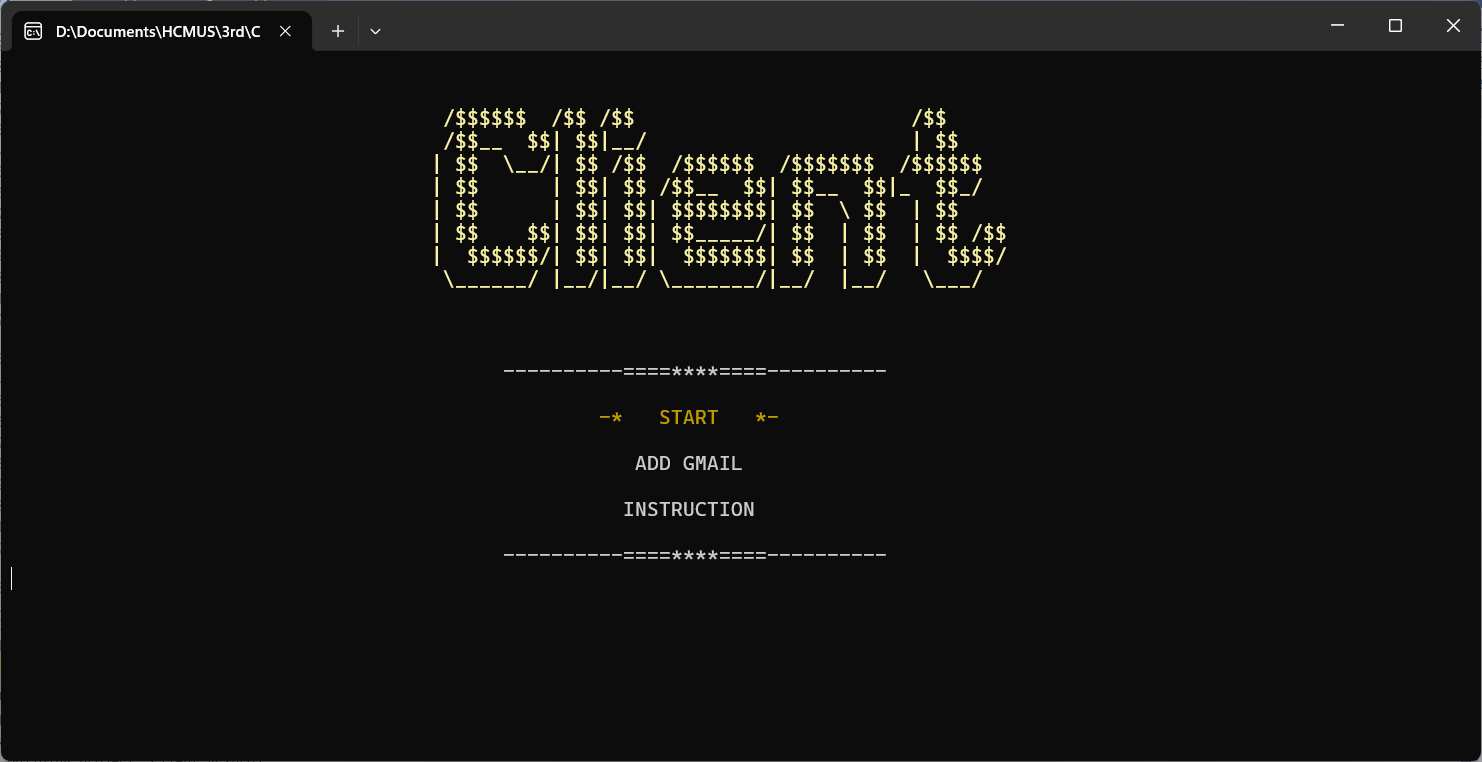
\includegraphics[width=0.7\textwidth]{img/client.png}
    \caption{Giao diện của client}
\end{figure}

\begin{figure}
    \centering
    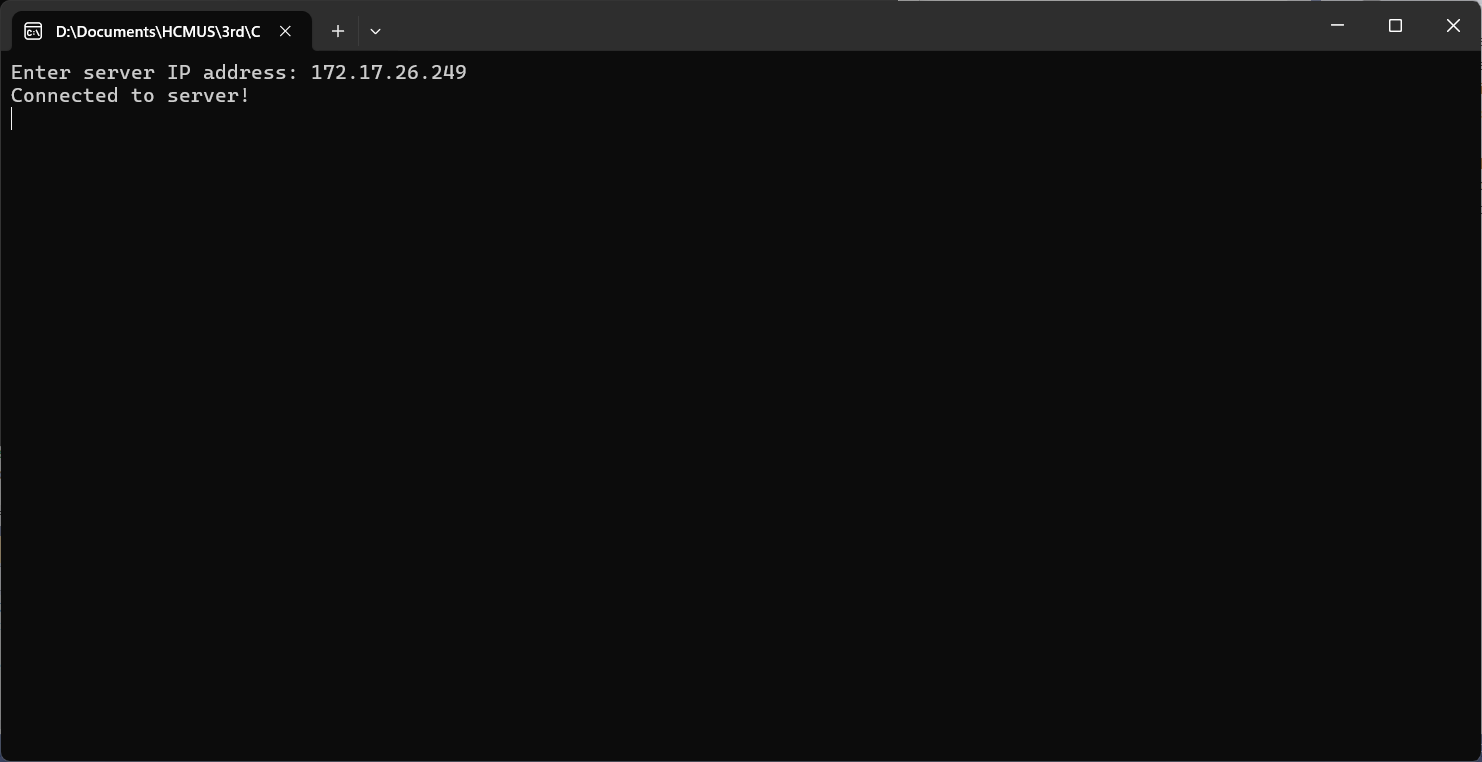
\includegraphics[width=0.7\textwidth]{img/start.png}
    \caption{Bắt đầu kết nối với server}
\end{figure}

\begin{figure}[H]
    \centering
    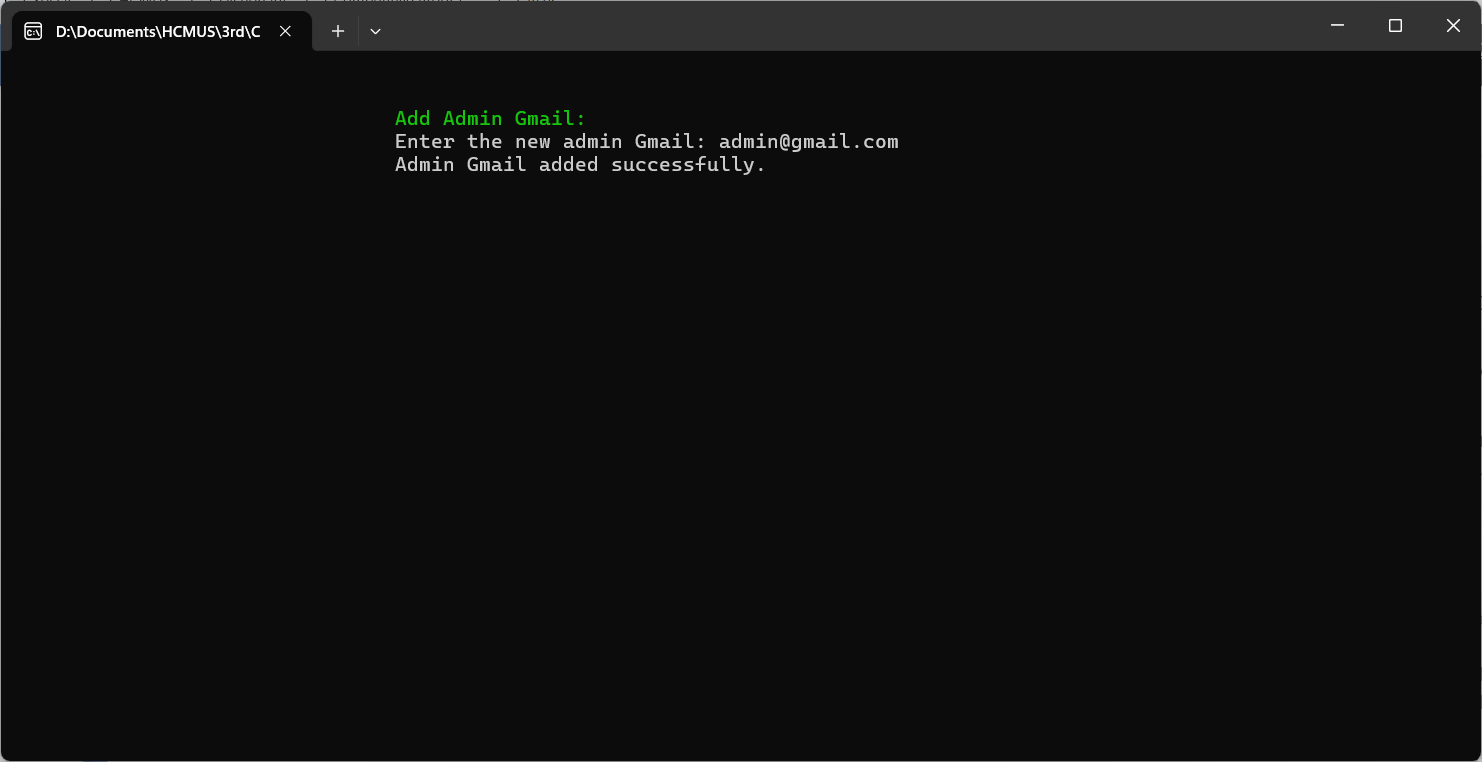
\includegraphics[width=0.7\textwidth]{img/add_gmail.png}
    \caption{Thêm tài khoản Gmail Admin}
\end{figure}

\begin{figure}[H]
    \centering
    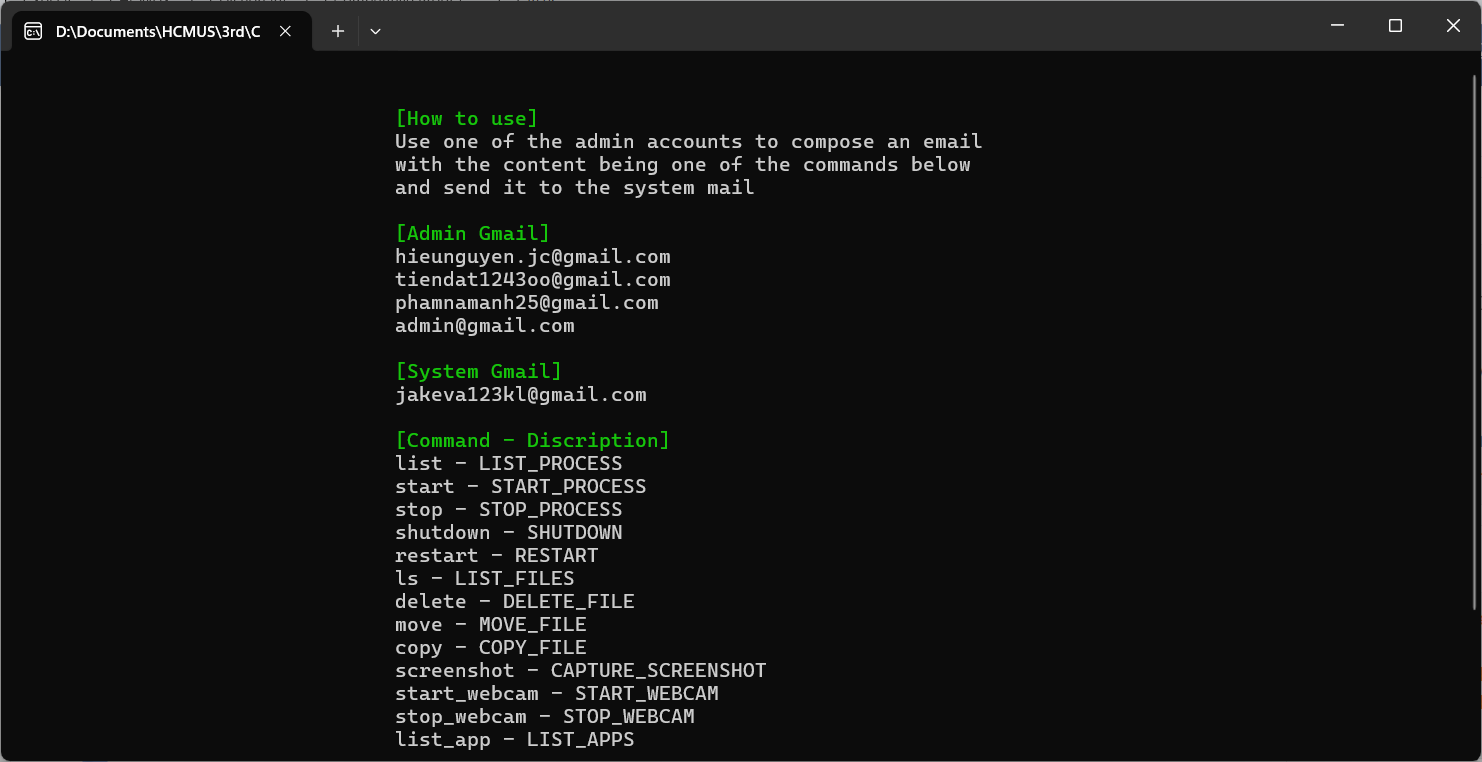
\includegraphics[width=0.7\textwidth]{img/instruction.png}
    \caption{Hướng dẫn sử dụng và các lệnh điều khiển}
\end{figure}

\subsubsection{Server}

Giao diện của server được viết trực tiếp trong hàm \texttt{void main()} hiển thị thông tin về server như IP, tình trạng kết nối với client, và các lệnh điều khiển, dưới đây là hình minh họa cho giao diện của server:

\begin{figure}[H]
    \centering
    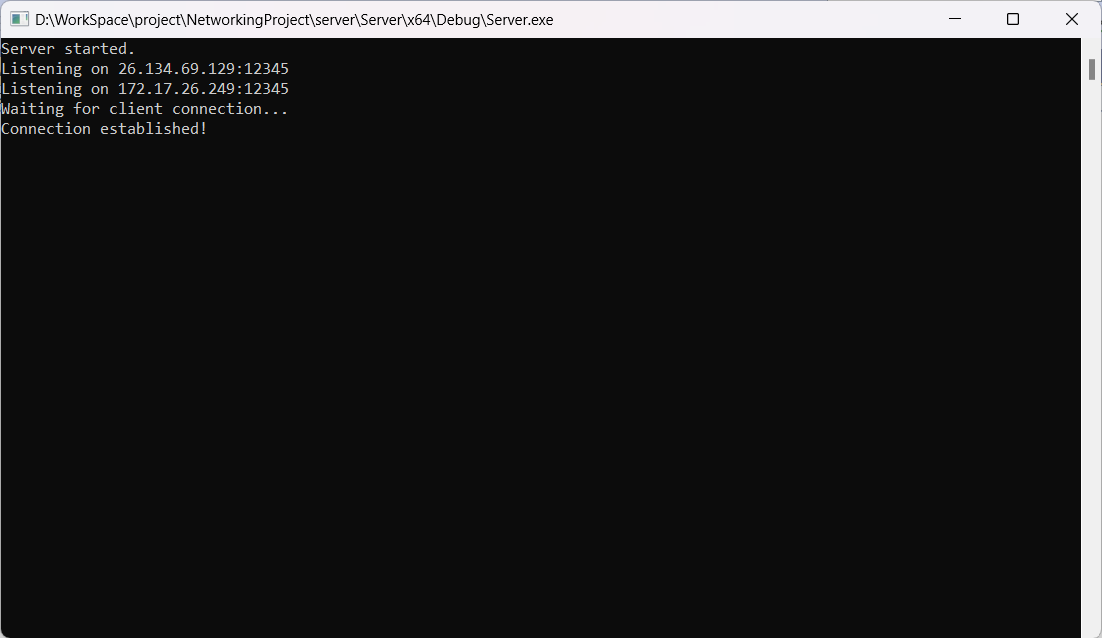
\includegraphics[width=0.7\textwidth]{img/server.png}
    \caption{Giao diện của server}
\end{figure}
\newpage

\subsection{Gmail API}
\subsubsection{Lấy Access Token}
\begin{itemize}
    \item \textbf{Tên hàm:} \texttt{std::string getAccessToken()}
    \item \textbf{Chức năng:} 
    \begin{itemize}
        \item Lấy access token từ Google OAuth 2.0 để sử dụng cho các yêu cầu API tiếp theo.
    \end{itemize}
    \item \textbf{Mục đích:} 
    \begin{itemize}
        \item Access token được sử dụng để xác thực các yêu cầu API đến Gmail. Đây là bước đầu tiên và quan trọng để có thể thực hiện các thao tác khác với Gmail API.
    \end{itemize}
    \item \textbf{Cách thức hoạt động:} 
    \begin{itemize}
        \item Hàm sử dụng thông tin xác thực đã cấu hình trước (client ID, client secret) để gửi yêu cầu đến máy chủ Google OAuth 2.0.
        \item Máy chủ trả về access token nếu thông tin xác thực hợp lệ.
    \end{itemize}
    \item \textbf{Tham số truyền vào:} 
    \begin{itemize}
        \item Không có tham số truyền vào.
    \end{itemize}
    \item \textbf{Tham số trả về:} 
    \begin{itemize}
        \item \texttt{std::string}: Chuỗi chứa access token.
    \end{itemize}
\end{itemize}

\subsubsection{Lấy Nội Dung Email}
\begin{itemize}
    \item \textbf{Tên hàm:} \texttt{std::string getEmail (const std::string\& accessToken, const \\std::string\& messageId)}
    \item \textbf{Chức năng:} 
    \begin{itemize}
        \item Lấy nội dung của một email dựa trên messageId.
    \end{itemize}
    \item \textbf{Mục đích:} 
    \begin{itemize}
        \item Đọc nội dung email từ Gmail. Sử dụng access token để xác thực và messageId để xác định email cụ thể cần đọc.
    \end{itemize}
    \item \textbf{Cách thức hoạt động:} 
    \begin{itemize}
        \item Hàm gửi yêu cầu HTTP GET đến Gmail API, bao gồm access token để xác thực và messageId để xác định email cần truy xuất.
        \item Gmail API trả về nội dung của email dưới dạng JSON, và hàm trích xuất nội dung từ phản hồi này.
    \end{itemize}
    \item \textbf{Tham số truyền vào:} 
    \begin{itemize}
        \item \texttt{accessToken}: Chuỗi chứa access token để xác thực yêu cầu API.
        \item \texttt{messageId}: Chuỗi chứa ID của email cần đọc.
    \end{itemize}
    \item \textbf{Tham số trả về:} 
    \begin{itemize}
        \item \texttt{std::string}: Chuỗi chứa nội dung của email.
    \end{itemize}
\end{itemize}

\subsubsection{Lấy ID Email Mới Nhất}
\begin{itemize}
    \item \textbf{Tên hàm:} \texttt{std::string getMessageId(const std::string\& accessToken)}
    \item \textbf{Chức năng:} 
    \begin{itemize}
        \item Lấy ID của email mới nhất trong hộp thư đến.
    \end{itemize}
    \item \textbf{Mục đích:} 
    \begin{itemize}
        \item Lấy ID của email để có thể đọc nội dung email đó. Giúp xác định email mới nhất mà người dùng nhận được.
    \end{itemize}
    \item \textbf{Cách thức hoạt động:} 
    \begin{itemize}
        \item Hàm gửi yêu cầu HTTP GET đến Gmail API, bao gồm access token để xác thực.
        \item Gmail API trả về danh sách email, và hàm trích xuất ID của email mới nhất từ danh sách này.
    \end{itemize}
    \item \textbf{Tham số truyền vào:} 
    \begin{itemize}
        \item \texttt{accessToken}: Chuỗi chứa access token để xác thực yêu cầu API.
    \end{itemize}
    \item \textbf{Tham số trả về:} 
    \begin{itemize}
        \item \texttt{std::string}: Chuỗi chứa ID của email mới nhất.
    \end{itemize}
\end{itemize}

\subsubsection{Kiểm Tra Email Từ Admin}
\begin{itemize}
    \item \textbf{Tên hàm:} \texttt{bool isAdmin(const std::string\& accessToken, const \\std::vector<std::string>\& adminMail, const std::string\& messageId, \\std::string\& senderMail)}
    \item \textbf{Chức năng:} 
    \begin{itemize}
        \item Kiểm tra xem email gửi đến có phải từ admin hay không.
    \end{itemize}
    \item \textbf{Mục đích:} 
    \begin{itemize}
        \item Xác định quyền admin của người gửi email. Đảm bảo rằng chỉ những email từ admin mới được xử lý.
    \end{itemize}
    \item \textbf{Cách thức hoạt động:} 
    \begin{itemize}
        \item Hàm sử dụng access token và messageId để lấy thông tin email.
        \item Hàm trích xuất địa chỉ email của người gửi từ nội dung email và so sánh với danh sách \texttt{adminMail}.
    \end{itemize}
    \item \textbf{Tham số truyền vào:} 
    \begin{itemize}
        \item \texttt{accessToken}: Chuỗi chứa access token để xác thực yêu cầu API.
        \item \texttt{adminMail}: Vector chứa danh sách các email admin.
        \item \texttt{messageId}: Chuỗi chứa ID của email cần kiểm tra.
        \item \texttt{senderMail}: Tham chiếu đến chuỗi để lưu email của người gửi nếu là admin.
    \end{itemize}
    \item \textbf{Tham số trả về:} 
    \begin{itemize}
        \item \texttt{bool}: Trả về \texttt{true} nếu email gửi đến từ admin, ngược lại trả về \texttt{false}.
    \end{itemize}
\end{itemize}

\subsubsection{Gửi Email Đơn Giản}
\begin{itemize}
    \item \textbf{Tên hàm:} \texttt{void sendEmail(const std::string\& accessToken, const std::string\& to, const std::string\& subject, const std::string\& body)}
    \item \textbf{Chức năng:} 
    \begin{itemize}
        \item Gửi một email đơn giản.
    \end{itemize}
    \item \textbf{Mục đích:} 
    \begin{itemize}
        \item Gửi email từ tài khoản Gmail. Sử dụng access token để xác thực và gửi email đến địa chỉ được chỉ định.
    \end{itemize}
    \item \textbf{Cách thức hoạt động:} 
    \begin{itemize}
        \item Hàm gửi yêu cầu HTTP POST đến Gmail API, bao gồm access token và thông tin email (người nhận, tiêu đề, nội dung).
        \item Gmail API xử lý yêu cầu và trả về kết quả gửi email.
    \end{itemize}
    \item \textbf{Tham số truyền vào:} 
    \begin{itemize}
        \item \texttt{accessToken}: Chuỗi chứa access token để xác thực yêu cầu API.
        \item \texttt{to}: Chuỗi chứa địa chỉ email của người nhận.
        \item \texttt{subject}: Chuỗi chứa tiêu đề của email.
        \item \texttt{body}: Chuỗi chứa nội dung của email.
    \end{itemize}
    \item \textbf{Tham số trả về:} 
    \begin{itemize}
        \item Không có tham số trả về.
    \end{itemize}
\end{itemize}

\subsubsection{Gửi Email Có Tệp Đính Kèm}
\begin{itemize}
    \item \textbf{Tên hàm:} \texttt{void sendGmailWithAttachment(const std::string\& accessToken, const \\std::string\& to, const std::string\& subject, const std::string\& body, const \\std::string\& attachmentPath)}
    \item \textbf{Chức năng:} 
    \begin{itemize}
        \item Gửi một email với tệp đính kèm.
    \end{itemize}
    \item \textbf{Mục đích:} 
    \begin{itemize}
        \item Gửi email từ tài khoản Gmail với tệp đính kèm. Sử dụng access token để xác thực và gửi email đến địa chỉ được chỉ định cùng với tệp đính kèm.
    \end{itemize}
    \item \textbf{Cách thức hoạt động:} 
    \begin{itemize}
        \item Hàm xây dựng email dưới dạng MIME message, bao gồm tiêu đề, nội dung, và tệp đính kèm.
        \item Hàm gửi yêu cầu HTTP POST đến Gmail API, bao gồm access token và MIME message.
        \item Gmail API xử lý yêu cầu và gửi email.
    \end{itemize}
    \item \textbf{Tham số truyền vào:} 
    \begin{itemize}
        \item \texttt{accessToken}: Chuỗi chứa access token để xác thực yêu cầu API.
        \item \texttt{to}: Chuỗi chứa địa chỉ email của người nhận.
        \item \texttt{subject}: Chuỗi chứa tiêu đề của email.
        \item \texttt{body}: Chuỗi chứa nội dung của email.
        \item \texttt{attachmentPath}: Chuỗi chứa đường dẫn đến tệp đính kèm.
    \end{itemize}
    \item \textbf{Tham số trả về:} 
    \begin{itemize}
        \item Không có tham số trả về.
    \end{itemize}
\end{itemize}

\subsubsection{Mã Hóa Base64}
\begin{itemize}
    \item \textbf{Tên hàm:} \texttt{std::string base64\_encode(const std::string\& input)}
    \item \textbf{Chức năng:} 
    \begin{itemize}
        \item Chuyển đổi chuỗi văn bản hoặc dữ liệu nhị phân thành định dạng base64.
    \end{itemize}
    \item \textbf{Mục đích:} 
    \begin{itemize}
        \item Base64 là định dạng mã hóa phổ biến dùng để truyền dữ liệu qua các giao thức không hỗ trợ dữ liệu nhị phân, ví dụ: email MIME hoặc HTTP.
    \end{itemize}
    \item \textbf{Cách thức hoạt động:} 
    \begin{itemize}
        \item Chuỗi đầu vào được chia thành các nhóm byte.
        \item Mỗi nhóm byte được ánh xạ thành các ký tự trong bảng base64.
        \item Kết quả cuối cùng được làm đầy bằng ký tự `=` để đảm bảo độ dài là bội số của 4.
    \end{itemize}
    \item \textbf{Tham số truyền vào:} 
    \begin{itemize}
        \item \texttt{input}: Chuỗi cần mã hóa.
    \end{itemize}
    \item \textbf{Tham số trả về:} 
    \begin{itemize}
        \item \texttt{std::string}: Chuỗi được mã hóa dưới dạng base64.
    \end{itemize}
\end{itemize}

\subsubsection{Giải Mã Base64}
\begin{itemize}
    \item \textbf{Tên hàm:} \texttt{std::string base64\_decode(const std::string\& input)}
    \item \textbf{Chức năng:} 
    \begin{itemize}
        \item Giải mã một chuỗi base64 thành dữ liệu hoặc chuỗi ban đầu.
    \end{itemize}
    \item \textbf{Mục đích:} 
    \begin{itemize}
        \item Khôi phục dữ liệu từ chuỗi base64 đã mã hóa. Thường được dùng khi xử lý email hoặc tệp đính kèm.
    \end{itemize}
    \item \textbf{Cách thức hoạt động:} 
    \begin{itemize}
        \item Các ký tự trong chuỗi base64 được ánh xạ ngược lại thành giá trị nhị phân.
        \item Các giá trị nhị phân được tổ hợp để khôi phục dữ liệu ban đầu.
    \end{itemize}
    \item \textbf{Tham số truyền vào:} 
    \begin{itemize}
        \item \texttt{input}: Chuỗi base64 cần giải mã.
    \end{itemize}
    \item \textbf{Tham số trả về:} 
    \begin{itemize}
        \item \texttt{std::string}: Chuỗi dữ liệu sau khi giải mã.
    \end{itemize}
\end{itemize}

\newpage

\subsection{Socket}
\subsubsection{Client}
\paragraph{\textbf{Khởi tạo Winsock}}
\begin{itemize}
    \item \textbf{Prototype:} \texttt{bool initializeWinsock(WSADATA\& wsaData);}
    
    \item \textbf{Mục đích:} Khởi tạo thư viện Winsock để sử dụng các API mạng.
    
    \item \textbf{Cách thức hoạt động:} 
    \begin{enumerate}
        \item Gọi hàm \texttt{WSAStartup()} để khởi tạo Winsock.
        \item Kiểm tra lỗi nếu việc khởi tạo thất bại.
    \end{enumerate}
    
    \item \textbf{Tham số truyền vào:} 
    \begin{itemize}
        \item \texttt{WSADATA\& wsaData}: Một cấu trúc chứa thông tin về phiên bản Winsock được khởi tạo.
    \end{itemize}
    
    \item \textbf{Tham số trả về:} \texttt{true} nếu khởi tạo thành công, \texttt{false} nếu thất bại.
\end{itemize}

\paragraph{\textbf{Nhập địa chỉ IP server}}
\begin{itemize}
    \item \textbf{Prototype:} \texttt{std::string getServerAddressInput();}
    
    \item \textbf{Mục đích:} Nhận địa chỉ IP của server từ người dùng.
    
    \item \textbf{Cách thức hoạt động:} 
    \begin{enumerate}
        \item Hiển thị lời nhắc yêu cầu người dùng nhập địa chỉ IP của server.
        \item Đọc địa chỉ IP từ bàn phím.
    \end{enumerate}
    
    \item \textbf{Tham số truyền vào:} Không có.
    
    \item \textbf{Tham số trả về:} Chuỗi chứa địa chỉ IP của server.
\end{itemize}

\paragraph{\textbf{Lấy thông tin địa chỉ server}}
\begin{itemize}
    \item \textbf{Prototype:} \texttt{addrinfo* getServerAddress(const std::string\& serverAddress, const std::string\& port, const addrinfo\& hints);}
    
    \item \textbf{Mục đích:} Lấy thông tin địa chỉ của server từ hệ thống.
    
    \item \textbf{Cách thức hoạt động:} 
    \begin{enumerate}
        \item Gọi hàm \texttt{getaddrinfo()} để lấy danh sách địa chỉ phù hợp với cấu hình.
        \item Kiểm tra lỗi và trả về danh sách địa chỉ hoặc thông báo lỗi nếu có.
    \end{enumerate}
    
    \item \textbf{Tham số truyền vào:} 
    \begin{itemize}
        \item \texttt{serverAddress}: Địa chỉ IP của server.
        \item \texttt{port}: Cổng mà server sử dụng.
        \item \texttt{hints}: Cấu hình tìm kiếm thông tin địa chỉ (ví dụ: loại giao thức, kiểu socket).
    \end{itemize}
    
    \item \textbf{Tham số trả về:} Con trỏ đến danh sách thông tin địa chỉ \texttt{addrinfo*}, hoặc \texttt{NULL} nếu thất bại.
\end{itemize}

\paragraph{\textbf{Kết nối đến server}}
\begin{itemize}
    \item \textbf{Prototype:} \texttt{bool connectToServer(SOCKET\& ConnectSocket, addrinfo* result);}
    
    \item \textbf{Mục đích:} Thiết lập kết nối từ Client đến Server.
    
    \item \textbf{Cách thức hoạt động:}
    \begin{enumerate}
        \item Lặp qua các địa chỉ trong danh sách \texttt{result}.
        \item Tạo socket với các thông tin địa chỉ phù hợp bằng hàm \texttt{socket()}.
        \item Thực hiện kết nối đến server bằng hàm \texttt{connect()}.
        \item Đóng socket nếu kết nối không thành công và thử địa chỉ tiếp theo.
    \end{enumerate}
    
    \item \textbf{Tham số truyền vào:}
    \begin{itemize}
        \item \texttt{ConnectSocket}: Socket sẽ được sử dụng để kết nối.
        \item \texttt{result}: Danh sách địa chỉ và cổng của server (từ hàm \texttt{getServerAddress()}).
    \end{itemize}
    
    \item \textbf{Tham số trả về:} \texttt{true} nếu kết nối thành công, \texttt{false} nếu thất bại.
\end{itemize}

\paragraph{\textbf{Gửi yêu cầu từ client}}
\begin{itemize}
    \item \textbf{Prototype:}\\ \texttt{bool sendClientRequest(SOCKET\& ConnectSocket, const std::string\& request);}
    
    \item \textbf{Mục đích:} Gửi yêu cầu từ client đến server qua socket.
    
    \item \textbf{Cách thức hoạt động:} 
    \begin{enumerate}
        \item Gửi chuỗi yêu cầu bằng hàm \texttt{send()}.
        \item Kiểm tra lỗi nếu việc gửi thất bại và hiển thị thông báo lỗi.
    \end{enumerate}
    
    \item \textbf{Tham số truyền vào:} 
    \begin{itemize}
        \item \texttt{ConnectSocket}: Socket kết nối đến server.
        \item \texttt{request}: Chuỗi yêu cầu cần gửi.
    \end{itemize}
    
    \item \textbf{Tham số trả về:} 
    \begin{itemize}
        \item \texttt{true} nếu gửi thành công.
        \item \texttt{false} nếu thất bại.
    \end{itemize}
\end{itemize}

\paragraph{\textbf{Nhận loại phản hồi từ server}}
\begin{itemize}
    \item \textbf{Prototype:} \texttt{std::string receiveResponseType(SOCKET\& ConnectSocket, char* recvbuf, int recvbuflen);}
    
    \item \textbf{Mục đích:} Xác định loại phản hồi từ server (văn bản hoặc tệp tin).
    
    \item \textbf{Cách thức hoạt động:} 
    \begin{enumerate}
        \item Nhận kích thước loại phản hồi qua \texttt{recv()}.
        \item Nhận dữ liệu mô tả loại phản hồi từ server.
        \item Kiểm tra lỗi trong quá trình nhận.
    \end{enumerate}
    
    \item \textbf{Tham số truyền vào:} 
    \begin{itemize}
        \item \texttt{ConnectSocket}: Socket kết nối đến server.
        \item \texttt{recvbuf}: Bộ đệm để nhận dữ liệu.
        \item \texttt{recvbuflen}: Kích thước bộ đệm.
    \end{itemize}
    
    \item \textbf{Tham số trả về:} Chuỗi xác định loại phản hồi (\texttt{"text"} hoặc \texttt{"file"}).
\end{itemize}

\paragraph{\textbf{Xử lý phản hồi dạng tệp}}
\begin{itemize}
    \item \textbf{Prototype:} \texttt{std::string handleFileResponse(SOCKET\& ConnectSocket, char* recvbuf, int recvbuflen);}
    
    \item \textbf{Mục đích:} Nhận và lưu trữ tệp tin được gửi từ server.
    
    \item \textbf{Cách thức hoạt động:} 
    \begin{enumerate}
        \item Nhận tên tệp và kích thước tệp từ server.
        \item Mở tệp để ghi dữ liệu.
        \item Nhận từng phần dữ liệu từ server và ghi vào tệp.
        \item Hiển thị thanh tiến trình trong quá trình nhận tệp.
        \item Đóng tệp sau khi hoàn tất.
    \end{enumerate}
    
    \item \textbf{Tham số truyền vào:} 
    \begin{itemize}
        \item \texttt{ConnectSocket}: Socket kết nối đến server.
        \item \texttt{recvbuf}: Bộ đệm để nhận dữ liệu.
        \item \texttt{recvbuflen}: Kích thước bộ đệm.
    \end{itemize}
    
    \item \textbf{Tham số trả về:} Tên của tệp tin đã nhận.
\end{itemize}

\paragraph{\textbf{Xử lý phản hồi dạng văn bản}}
\begin{itemize}
    \item \textbf{Prototype:} \texttt{std::string handleTextResponse(SOCKET\& ConnectSocket, char* recvbuf, int recvbuflen);}
    
    \item \textbf{Mục đích:} Nhận phản hồi dạng văn bản từ server và in ra màn hình.
    
    \item \textbf{Cách thức hoạt động:} 
    \begin{enumerate}
        \item Nhận kích thước phản hồi từ server.
        \item Nhận từng phần của phản hồi và lưu vào bộ đệm.
        \item In phản hồi ra màn hình.
    \end{enumerate}
    
    \item \textbf{Tham số truyền vào:} 
    \begin{itemize}
        \item \texttt{ConnectSocket}: Socket kết nối đến server.
        \item \texttt{recvbuf}: Bộ đệm để nhận dữ liệu.
        \item \texttt{recvbuflen}: Kích thước bộ đệm.
    \end{itemize}
    
    \item \textbf{Tham số trả về:} Chuỗi phản hồi từ server.
\end{itemize}

\paragraph{\textbf{Vòng lặp giao tiếp}}
\begin{itemize}
    \item \textbf{Prototype:} \texttt{void chatLoop(SOCKET\& ConnectSocket, char* recvbuf, int recvbuflen);}
    
    \item \textbf{Mục đích:} Thực hiện vòng lặp giao tiếp liên tục giữa client và server.
    
    \item \textbf{Cách thức hoạt động:} 
    \begin{enumerate}
        \item Lấy yêu cầu từ email (tích hợp với Gmail API).
        \item Gửi yêu cầu đến server bằng hàm \texttt{sendClientRequest()}.
        \item Nhận phản hồi từ server:
        \begin{itemize}
            \item Nếu phản hồi là tệp, sử dụng hàm \texttt{handleFileResponse()} để lưu tệp.
            \item Nếu phản hồi là văn bản, sử dụng hàm \texttt{handleTextResponse()} để hiển thị.
        \end{itemize}
        \item Gửi phản hồi lại email người gửi thông qua Gmail API.
        \item Lặp lại sau mỗi 10 giây hoặc thoát nếu yêu cầu là \texttt{"exit"}.
    \end{enumerate}
    
    \item \textbf{Tham số truyền vào:} 
    \begin{itemize}
        \item \texttt{ConnectSocket}: Socket kết nối đến server.
        \item \texttt{recvbuf}: Bộ đệm để nhận dữ liệu.
        \item \texttt{recvbuflen}: Kích thước bộ đệm.
    \end{itemize}
    
    \item \textbf{Tham số trả về:} Không có.
\end{itemize}

\paragraph{\textbf{Dọn dẹp tài nguyên}}
\begin{itemize}
    \item \textbf{Prototype:} \texttt{void cleanup(SOCKET\& ConnectSocket);}
    
    \item \textbf{Mục đích:} Giải phóng tài nguyên socket và thư viện Winsock.
    
    \item \textbf{Cách thức hoạt động:} 
    \begin{enumerate}
        \item Đóng socket bằng \texttt{closesocket()}.
        \item Gọi \texttt{WSACleanup()} để giải phóng Winsock.
    \end{enumerate}
    
    \item \textbf{Tham số truyền vào:} 
    \begin{itemize}
        \item \texttt{ConnectSocket}: Socket đã sử dụng.
    \end{itemize}
    
    \item \textbf{Tham số trả về:} Không có.
\end{itemize}

\paragraph{\textbf{Khởi động Client}}
\begin{itemize}
    \item \textbf{Prototype:} \texttt{void startClient();}
    
    \item \textbf{Mục đích:} Thiết lập một client sử dụng Winsock để kết nối đến server qua giao thức TCP, sau đó thực hiện giao tiếp giữa client và server.
    
    \item \textbf{Cách thức hoạt động:} 
    \begin{enumerate}
        \item Khởi tạo Winsock bằng cách gọi hàm \texttt{initializeWinsock}.
        \item Cấu hình các tham số của socket bằng cách sử dụng cấu trúc \texttt{addrinfo}:
        \begin{itemize}
            \item \texttt{ai\_family}: Được đặt là \texttt{AF\_UNSPEC}, cho phép sử dụng cả IPv4 và IPv6.
            \item \texttt{ai\_socktype}: Được đặt là \texttt{SOCK\_STREAM}, sử dụng giao thức TCP.
            \item \texttt{ai\_protocol}: Được đặt là \texttt{IPPROTO\_TCP}, chỉ định giao thức TCP.
        \end{itemize}
        \item Thực hiện vòng lặp kết nối:
        \begin{itemize}
            \item Yêu cầu người dùng nhập địa chỉ IP của server.
            \item Sử dụng hàm \texttt{getServerAddress} để giải quyết địa chỉ server và cổng.
            \item Nếu không thể kết nối, hiển thị thông báo lỗi và cho phép người dùng nhập lại địa chỉ IP.
            \item Nếu kết nối thành công, hiển thị thông báo kết nối thành công.
        \end{itemize}
        \item Sau khi kết nối thành công, thực hiện giao tiếp giữa client và server bằng cách gọi hàm \texttt{chatLoop}.
        \item Dọn dẹp tài nguyên và đóng kết nối bằng cách gọi hàm \texttt{cleanup}.
    \end{enumerate}
    
    \item \textbf{Tham số truyền vào:} Không có.
    
    \item \textbf{Tham số trả về:} Không có.
\end{itemize}


\paragraph{\textbf{In thanh tiến trình}}
\begin{itemize}
    \item \textbf{Prototype:} \texttt{void printProgressBar(int progress, int total);}
    
    \item \textbf{Mục đích:} In thanh tiến trình lên màn hình để hiển thị tỷ lệ hoàn thành công việc.
    
    \item \textbf{Cách thức hoạt động:} 
    \begin{enumerate}
        \item Tính toán tỷ lệ phần trăm dựa trên tiến độ (\texttt{progress}) và tổng số công việc (\texttt{total}).
        \item Xử lý việc hiển thị thanh tiến trình với chiều rộng cố định.
        \item Hiển thị ký tự \texttt{=} cho các phần đã hoàn thành và ký tự \texttt{>} cho phần hiện tại.
        \item Cập nhật thanh tiến trình liên tục trong quá trình công việc diễn ra.
    \end{enumerate}

    \item \textbf{Tham số truyền vào:} 
    \begin{itemize}
        \item \texttt{progress}: Số lượng công việc đã hoàn thành.
        \item \texttt{total}: Tổng số công việc cần hoàn thành.
    \end{itemize}
    
    \item \textbf{Tham số trả về:} Không có.
\end{itemize}

% Server
\subsubsection{Server}

\paragraph{\textbf{Khởi tạo Winsock}}
\begin{itemize}
    \item \textbf{Prototype:} \texttt{bool initializeWinsock(WSADATA\& wsaData);}
    
    \item \textbf{Mục đích:} Khởi tạo thư viện Winsock để sử dụng các API mạng.
    
    \item \textbf{Cách thức hoạt động:} 
    \begin{enumerate}
        \item Gọi hàm \texttt{WSAStartup()} để khởi tạo Winsock.
        \item Kiểm tra lỗi nếu việc khởi tạo thất bại.
    \end{enumerate}
    
    \item \textbf{Tham số truyền vào:} 
    \begin{itemize}
        \item \texttt{WSADATA\& wsaData}: Một cấu trúc chứa thông tin về phiên bản Winsock được khởi tạo.
    \end{itemize}
    
    \item \textbf{Tham số trả về:} \texttt{true} nếu khởi tạo thành công, \texttt{false} nếu thất bại.
\end{itemize}

\paragraph{\textbf{Cấu hình socket}}
\begin{itemize}
    \item \textbf{Prototype:} \texttt{bool setupSocket(SOCKET\& ListenSocket, addrinfo*\& result);}
    
    \item \textbf{Mục đích:} Tạo và cấu hình socket để chấp nhận kết nối từ client.
    
    \item \textbf{Cách thức hoạt động:} 
    \begin{enumerate}
        \item Thiết lập thông tin cấu hình cho socket sử dụng \texttt{addrinfo}.
        \item Gọi hàm \texttt{getaddrinfo()} để lấy thông tin cấu hình.
        \item Tạo socket bằng \texttt{socket()}.
        \item Gắn socket với địa chỉ và cổng bằng \texttt{bind()}.
        \item Bắt đầu lắng nghe kết nối bằng \texttt{listen()}.
    \end{enumerate}
    
    \item \textbf{Tham số truyền vào:} 
    \begin{itemize}
        \item \texttt{SOCKET\& ListenSocket}: Biến tham chiếu đại diện cho socket server.
        \item \texttt{addrinfo*\& result}: Con trỏ lưu trữ thông tin cấu hình socket.
    \end{itemize}
    
    \item \textbf{Tham số trả về:} \texttt{true} nếu cấu hình thành công, \texttt{false} nếu thất bại.
\end{itemize}

\paragraph{\textbf{In thông tin địa chỉ IP}}
\begin{itemize}
    \item \textbf{Prototype:} \texttt{void printIPAddress(const sockaddr\_in\& addr);}
    
    \item \textbf{Mục đích:} Hiển thị địa chỉ IP và cổng mà server đang lắng nghe.
    
    \item \textbf{Cách thức hoạt động:} 
    \begin{enumerate}
        \item Sử dụng lệnh \texttt{ipconfig} để lấy thông tin địa chỉ IP.
        \item Phân tích dữ liệu đầu ra để tìm địa chỉ IPv4.
        \item Hiển thị thông tin địa chỉ IP và cổng.
    \end{enumerate}
    
    \item \textbf{Tham số truyền vào:} 
    \begin{itemize}
        \item \texttt{const sockaddr\_in\& addr}: Cấu trúc chứa thông tin địa chỉ IP và cổng.
    \end{itemize}
    
    \item \textbf{Tham số trả về:} Không có.
\end{itemize}

\paragraph{\textbf{Hiển thị thông tin lắng nghe của socket}}
\begin{itemize}
    \item \textbf{Prototype:} \texttt{void printListeningInfo(SOCKET\& ListenSocket);}
    
    \item \textbf{Mục đích:} Hiển thị thông tin về địa chỉ IP và cổng mà server đang lắng nghe.
    
    \item \textbf{Cách thức hoạt động:} 
    \begin{enumerate}
        \item Lấy thông tin địa chỉ liên kết với socket bằng \texttt{getsockname()}.
        \item Chuyển đổi địa chỉ IP từ dạng nhị phân sang dạng chuỗi bằng \texttt{inet\_ntop()}.
        \item In thông tin địa chỉ IP và cổng ra màn hình.
    \end{enumerate}
    
    \item \textbf{Tham số truyền vào:} 
    \begin{itemize}
        \item \texttt{SOCKET\& ListenSocket}: Biến tham chiếu đại diện cho socket đang lắng nghe kết nối.
    \end{itemize}
    
    \item \textbf{Tham số trả về:} Không có.
\end{itemize}

\paragraph{\textbf{Chấp nhận kết nối từ client}}
\begin{itemize}
    \item \textbf{Prototype:} \texttt{SOCKET acceptClient(SOCKET\& ListenSocket);}
    
    \item \textbf{Mục đích:} Chấp nhận kết nối từ một client.
    
    \item \textbf{Cách thức hoạt động:} 
    \begin{enumerate}
        \item Gọi hàm \texttt{accept()} để chấp nhận kết nối từ client.
        \item Kiểm tra lỗi nếu việc chấp nhận kết nối thất bại.
    \end{enumerate}
    
    \item \textbf{Tham số truyền vào:} 
    \begin{itemize}
        \item \texttt{SOCKET\& ListenSocket}: Biến tham chiếu đại diện cho socket server đang lắng nghe.
    \end{itemize}
    
    \item \textbf{Tham số trả về:} Socket đại diện cho kết nối với client hoặc \texttt{INVALID\_SOCKET} nếu thất bại.
\end{itemize}

\paragraph{\textbf{Xử lý yêu cầu từ client}}
\begin{itemize}
    \item \textbf{Prototype:} \texttt{void processRequest(SOCKET\& ClientSocket, std::string\& request);}
    
    \item \textbf{Mục đích:} Xử lý yêu cầu từ client và trả về phản hồi phù hợp.
    
    \item \textbf{Cách thức hoạt động:} 
    \begin{enumerate}
        \item Loại bỏ ký tự không mong muốn khỏi yêu cầu.
        \item Phân tích cú pháp yêu cầu để xác định lệnh và tham số.
        \item Gọi hàm xử lý tương ứng dựa trên lệnh nhận được.
        \item Gửi phản hồi hoặc tệp tin đến client.
    \end{enumerate}
    
    \item \textbf{Tham số truyền vào:} 
    \begin{itemize}
        \item \texttt{SOCKET\& ClientSocket}: Biến tham chiếu đại diện cho kết nối với client.
        \item \texttt{std::string\& request}: Chuỗi chứa yêu cầu từ client.
    \end{itemize}
    
    \item \textbf{Tham số trả về:} Không có.
\end{itemize}

\paragraph{\textbf{Gửi tệp tin}}
\begin{itemize}
    \item \textbf{Prototype:} \texttt{void sendFile(SOCKET\& ClientSocket, std::string command);}
    
    \item \textbf{Mục đích:} Gửi tệp tin yêu cầu từ server đến client.
    
    \item \textbf{Cách thức hoạt động:} 
    \begin{enumerate}
        \item Xác định loại phản hồi và gửi thông tin này đến client.
        \item Lấy tên tệp tin từ lệnh yêu cầu.
        \item Gửi tên tệp, kích thước tệp và dữ liệu tệp đến client.
        \item Sử dụng \texttt{TransmitFile()} để gửi dữ liệu tệp.
    \end{enumerate}
    
    \item \textbf{Tham số truyền vào:} 
    \begin{itemize}
        \item \texttt{SOCKET\& ClientSocket}: Biến tham chiếu đại diện cho kết nối với client.
        \item \texttt{std::string command}: Lệnh chứa tên tệp tin cần gửi.
    \end{itemize}
    
    \item \textbf{Tham số trả về:} Không có.
\end{itemize}

\paragraph{\textbf{Gửi phản hồi}}
\begin{itemize}
    \item \textbf{Prototype:} \texttt{void sendResponse(SOCKET\& ClientSocket, std::string\& response);}
    
    \item \textbf{Mục đích:} Gửi phản hồi dạng văn bản đến client.
    
    \item \textbf{Cách thức hoạt động:} 
    \begin{enumerate}
        \item Xác định loại phản hồi là văn bản.
        \item Gửi kích thước và nội dung phản hồi đến client.
        \item Xử lý lỗi nếu quá trình gửi thất bại.
    \end{enumerate}
    
    \item \textbf{Tham số truyền vào:} 
    \begin{itemize}
        \item \texttt{SOCKET\& ClientSocket}: Biến tham chiếu đại diện cho kết nối với client.
        \item \texttt{std::string\& response}: Chuỗi chứa phản hồi cần gửi.
    \end{itemize}
    
    \item \textbf{Tham số trả về:} Không có.
\end{itemize}

\paragraph{\textbf{Xử lý kết nối từ client}}
\begin{itemize}
    \item \textbf{Prototype:} \texttt{void handleClient(SOCKET\& ClientSocket);}
    
    \item \textbf{Mục đích:} Quản lý và xử lý kết nối với một client.
    
    \item \textbf{Cách thức hoạt động:} 
    \begin{enumerate}
        \item Lắng nghe dữ liệu từ client.
        \item Phân tích và xử lý yêu cầu từ client.
        \item Đóng kết nối khi client gửi yêu cầu \texttt{exit} hoặc khi lỗi xảy ra.
    \end{enumerate}
    
    \item \textbf{Tham số truyền vào:} 
    \begin{itemize}
        \item \texttt{SOCKET\& ClientSocket}: Biến tham chiếu đại diện cho kết nối với client.
    \end{itemize}
    
    \item \textbf{Tham số trả về:} Không có.
\end{itemize}

\paragraph{\textbf{Dọn dẹp tài nguyên}}
\begin{itemize}
    \item \textbf{Prototype:} \texttt{void cleanup(SOCKET\& ClientSocket);}
    
    \item \textbf{Mục đích:} Dọn dẹp tài nguyên liên quan đến socket và Winsock.
    
    \item \textbf{Cách thức hoạt động:} 
    \begin{enumerate}
        \item Đóng socket sử dụng \texttt{closesocket()}.
        \item Giải phóng thư viện Winsock bằng \texttt{WSACleanup()}.
    \end{enumerate}
    
    \item \textbf{Tham số truyền vào:} 
    \begin{itemize}
        \item \texttt{SOCKET\& ClientSocket}: Biến tham chiếu đại diện cho kết nối với client.
    \end{itemize}
    \item \textbf{Tham số trả về:} Không có.
\end{itemize}

\paragraph{\textbf{Khởi động Server}}
\begin{itemize}
    \item \textbf{Prototype:} \texttt{void startServer();}
    
    \item \textbf{Mục đích:} Thiết lập một server cơ bản sử dụng thư viện Winsock để lắng nghe và xử lý kết nối từ client.
    
    \item \textbf{Cách thức hoạt động:} 
    \begin{enumerate}
        \item Khởi tạo Winsock bằng cách gọi hàm \texttt{initializeWinsock} để chuẩn bị môi trường làm việc.
        \item Thiết lập socket bằng cách:
        \begin{itemize}
            \item Giải quyết địa chỉ server với cấu trúc \texttt{addrinfo}.
            \item Tạo socket lắng nghe (\texttt{ListenSocket}) và liên kết với địa chỉ IP và cổng.
        \end{itemize}
        \item In thông tin lắng nghe để xác nhận server đã sẵn sàng nhận kết nối.
        \item Chấp nhận kết nối từ client bằng cách gọi \texttt{acceptClient}.
        \item Đóng socket lắng nghe (\texttt{ListenSocket}) vì không còn cần thiết sau khi kết nối đã được thiết lập.
        \item Xử lý giao tiếp với client bằng cách gọi hàm \texttt{handleClient}.
        \item Dọn dẹp tài nguyên và đóng kết nối sau khi hoàn thành.
    \end{enumerate}
    
    \item \textbf{Tham số truyền vào:} Không có.
    
    \item \textbf{Tham số trả về:} Không có.
\end{itemize}

\paragraph{\textbf{Xử lý lệnh từ client}}
\begin{itemize}
    \item \textbf{Prototype:} \texttt{static void handleRequest(const std::string\& request, std::string\& response, std::string\& params, std::ifstream\& file);}
    \item \textbf{Mục đích:} Xử lý yêu cầu từ client và trả về phản hồi phù hợp.
    \item \textbf{Cách thức hoạt động:}
          \begin{enumerate}
            \item Phân tích yêu cầu để xác định lệnh và tham số.
            \item Gọi hàm xử lý tương ứng dựa trên lệnh nhận được.
            \item Ghi phản hồi vào chuỗi \texttt{response}.
            \item Xử lý lỗi nếu có trong quá trình xử lý yêu cầu.
          \end{enumerate}
    \item \textbf{Tham số truyền vào:}
    \begin{itemize}
        \item \texttt{const std::string\& request}: Chuỗi yêu cầu từ client.
        \item \texttt{std::string\& response}: Chuỗi chứa phản hồi trả về client.
        \item \texttt{std::string\& params}: Chuỗi chứa tham số từ yêu cầu.
        \item \texttt{std::ifstream\& file}: Đối tượng file để đọc dữ liệu từ tệp tin.
    \end{itemize}
    \item \textbf{Tham số trả về:} Không có.
\end{itemize}
\newpage

\subsection{Các chức năng}
\subsubsection{Process}
\label{subsec:process}

\paragraph{List Processes}
\begin{itemize}
    \item \textbf{Tên hàm:} \texttt{bool listProcess(std::string \&result)}
    \item \textbf{Chức năng:}
    \begin{itemize}
        \item Liệt kê tất cả các process đang chạy trên máy.
    \end{itemize}
    \item \textbf{Mục đích:}
    \begin{itemize}
        \item Thông báo cho admin biết các process đang chạy trên máy.
    \end{itemize}
    \item \textbf{Cách thức hoạt động:}
    \begin{enumerate}
        \item Chạy lệnh liệt kê process trên hệ điều hành và lưu output.
        \item Trả về output cho hàm gọi.
    \end{enumerate}
    \item \textbf{Tham số truyền vào:}
    \begin{itemize}
        \item \texttt{result}: Chuỗi kết quả sau khi liệt kê process.
    \end{itemize}
    \item \textbf{Tham số trả về:}
    \begin{itemize}
        \item \texttt{bool}: Trả về \texttt{true} nếu thành công, \texttt{false} nếu thất bại.
    \end{itemize}
\end{itemize}

\paragraph{Start Process}
\begin{itemize}
    \item \textbf{Tên hàm:} \texttt{bool startProcess(std::string \&processName, std::string \&result)}
    \item \textbf{Chức năng:}
    \begin{itemize}
        \item Khởi động một process trên máy.
    \end{itemize}
    \item \textbf{Mục đích:}
    \begin{itemize}
        \item Thực thi một ứng dụng hoặc script trên máy.
    \end{itemize}
    \item \textbf{Cách thức hoạt động:}
    \begin{enumerate}
        \item Chạy lệnh khởi động process theo
        \item Trả về kết quả cho hàm gọi.
    \end{enumerate}
    \item \textbf{Tham số truyền vào:}
    \begin{itemize}
        \item \texttt{processName}: Tên/đường dẫn process cần khởi động.
        \item \texttt{result}: Chuỗi kết quả sau khi khởi động process.
    \end{itemize}
    \item \textbf{Tham số trả về:}
    \begin{itemize}
        \item \texttt{bool}: Trả về \texttt{true} nếu thành công, \texttt{false} nếu thất bại.
    \end{itemize}
\end{itemize}

\paragraph{Kill Process}
\begin{itemize}
    \item \textbf{Tên hàm:} \texttt{bool killProcess(std::string \&processName, std::string \&result)}
    \item \textbf{Chức năng:}
    \begin{itemize}
        \item Dừng một process đang chạy trên máy.
    \end{itemize}
    \item \textbf{Mục đích:}
    \begin{itemize}
        \item Dừng một ứng dụng hoặc script đang chạy trên máy.
    \end{itemize}
    \item \textbf{Cách thức hoạt động:}
    \begin{enumerate}
        \item Chạy lệnh dừng process theo \texttt{processName}.
        \item Trả về kết quả cho hàm gọi.
    \end{enumerate}
    \item \textbf{Tham số truyền vào:}
    \begin{itemize}
        \item \texttt{processName}: Tên/đường dẫn process cần dừng.
        \item \texttt{result}: Chuỗi kết quả sau khi dừng process.
    \end{itemize}
    \item \textbf{Tham số trả về:}
    \begin{itemize}
        \item \texttt{bool}: Trả về \texttt{true} nếu thành công, \texttt{false} nếu thất bại.
    \end{itemize}
\end{itemize}

\subsubsection{App}
\label{subsec:app}

\paragraph{List Applications}
\begin{itemize}
    \item \textbf{Tên hàm:} \texttt{bool listApps(std::string \&result)}
    \item \textbf{Chức năng:}
    \begin{itemize}
        \item Liệt kê tất cả các ứng dụng cài đặt trên máy.
    \end{itemize}
    \item \textbf{Mục đích:}
    \begin{itemize}
        \item Thông báo cho admin biết các ứng dụng cài đặt trên máy.
    \end{itemize}
    \item \textbf{Cách thức hoạt động:}
    \begin{enumerate}
        \item Duyệt thư mục lưu các shortcut ứng dụng trên máy.
        \item Đọc thông tin ứng dụng từ shortcut và lấy tên ứng dụng.
        \item Trả về tên các ứng dụng cho hàm gọi.
    \end{enumerate}
    \item \textbf{Tham số truyền vào:}
    \begin{itemize}
        \item \texttt{result}: Chuỗi kết quả sau khi liệt kê ứng dụng.
    \end{itemize}
    \item \textbf{Tham số trả về:}
    \begin{itemize}
        \item \texttt{bool}: Trả về \texttt{true} nếu thành công, \texttt{false} nếu thất bại.
    \end{itemize}
\end{itemize}

\paragraph{Start Application}
\begin{itemize}
    \item \textbf{Tên hàm:} \texttt{bool startApp(std::string \&appName, std::string \&result)}
    \item \textbf{Chức năng:}
    \begin{itemize}
        \item Khởi động một ứng dụng trên máy.
    \end{itemize}
    \item \textbf{Mục đích:}
    \begin{itemize}
        \item Mở một ứng dụng cụ thể trên máy.
    \end{itemize}
    \item \textbf{Cách thức hoạt động:}
    \begin{enumerate}
        \item Tìm shortcut của ứng dụng theo \texttt{appName}.
        \item Trích xuất đường dẫn ứng dụng từ shortcut.
        \item Chạy lệnh khởi động ứng dụng theo đường dẫn.
        \item Trả về kết quả cho hàm gọi.
    \end{enumerate}
    \item \textbf{Tham số truyền vào:}
    \begin{itemize}
        \item \texttt{appName}: Tên ứng dụng cần khởi động.
        \item \texttt{result}: Chuỗi kết quả sau khi khởi động ứng dụng.
    \end{itemize}
    \item \textbf{Tham số trả về:}
    \begin{itemize}
        \item \texttt{bool}: Trả về \texttt{true} nếu thành công, \texttt{false} nếu thất bại.
    \end{itemize}
\end{itemize}

\paragraph{Stop Application}
\begin{itemize}
    \item \textbf{Tên hàm:} \texttt{bool stopApp(std::string \&appName, std::string \&result)}
    \item \textbf{Chức năng:}
    \begin{itemize}
        \item Dừng một ứng dụng đang chạy trên máy.
    \end{itemize}
    \item \textbf{Mục đích:}
    \begin{itemize}
        \item Dừng một ứng dụng cụ thể đang chạy trên máy.
    \end{itemize}
    \item \textbf{Cách thức hoạt động:}
    \begin{enumerate}
        \item Tìm shortcut của ứng dụng theo \texttt{appName}.
        \item Trích xuất đường dẫn ứng dụng từ shortcut.
        \item Dừng ứng dụng theo đường dẫn.
        \item Trả về kết quả cho hàm gọi.
    \end{enumerate}
    \item \textbf{Tham số truyền vào:}
    \begin{itemize}
        \item \texttt{appName}: Tên ứng dụng cần dừng.
        \item \texttt{result}: Chuỗi kết quả sau khi dừng ứng dụng.
    \end{itemize}
    \item \textbf{Tham số trả về:}
    \begin{itemize}
        \item \texttt{bool}: Trả về \texttt{true} nếu thành công, \texttt{false} nếu thất bại.
    \end{itemize}
\end{itemize}

\subsubsection{Filesystem}
\label{subsec:filesystem}

\paragraph{List Files}
\begin{itemize}
    \item \textbf{Tên hàm:} \texttt{bool listFiles(std::string \&directory, std::string \&result)}
    \item \textbf{Chức năng:}
    \begin{itemize}
        \item Liệt kê tất cả các file và thư mục trong một thư mục.
    \end{itemize}
    \item \textbf{Mục đích:}
    \begin{itemize}
        \item Thông báo cho admin biết các file và thư mục trong một thư mục.
    \end{itemize}
    \item \textbf{Cách thức hoạt động:}
    \begin{enumerate}
        \item Chạy lệnh liệt kê file và thư mục trong thư mục \texttt{directory} trên hệ điều hành và lưu output.
        \item Đánh dấu file và thư mục trong output.
        \item Trả về output cho hàm gọi.
    \end{enumerate}
    \item \textbf{Tham số truyền vào:}
    \begin{itemize}
        \item \texttt{directory}: Đường dẫn thư mục cần liệt kê.
        \item \texttt{result}: Chuỗi kết quả sau khi liệt kê file và thư mục.
    \end{itemize}
    \item \textbf{Tham số trả về:}
    \begin{itemize}
        \item \texttt{bool}: Trả về \texttt{true} nếu thành công, \texttt{false} nếu thất bại.
    \end{itemize}
\end{itemize}

\paragraph{Delete File}
\begin{itemize}
    \item \textbf{Tên hàm:} \texttt{bool deleteFile(std::string \&fileName, std::string \&result)}
    \item \textbf{Chức năng:}
    \begin{itemize}
        \item Xóa một file hoặc thư mục trên máy.
    \end{itemize}
    \item \textbf{Mục đích:}
    \begin{itemize}
        \item Xóa một file hoặc thư mục không cần thiết trên máy.
    \end{itemize}
    \item \textbf{Cách thức hoạt động:}
    \begin{enumerate}
        \item Chạy lệnh xóa file hoặc thư mục theo \texttt{fileName}.
        \item Trả về kết quả cho hàm gọi.
    \end{enumerate}
    \item \textbf{Tham số truyền vào:}
    \begin{itemize}
        \item \texttt{filePath}: Đường dẫn file hoặc thư mục cần xóa.
        \item \texttt{result}: Chuỗi kết quả sau khi xóa file hoặc thư mục.
    \end{itemize}
    \item \textbf{Tham số trả về:}
    \begin{itemize}
        \item \texttt{bool}: Trả về \texttt{true} nếu thành công, \texttt{false} nếu thất bại.
    \end{itemize}
\end{itemize}

\paragraph{Copy File}
\begin{itemize}
    \item \textbf{Tên hàm:} \texttt{bool copyFile(std::string \&fileNames, std::string \&result)}
    \item \textbf{Chức năng:}
    \begin{itemize}
        \item Sao chép một file từ một thư mục đến một thư mục khác.
    \end{itemize}
    \item \textbf{Mục đích:}
    \begin{itemize}
        \item Sao chép một file từ một thư mục đến một thư mục khác.
    \end{itemize}
    \item \textbf{Cách thức hoạt động:}
    \begin{enumerate}
        \item Tách chuỗi \texttt{fileNames} thành \texttt{source} và \texttt{destination}.
        \item Chạy lệnh sao chép file từ \texttt{source} sang \texttt{destination}.
        \item Trả về kết quả cho hàm gọi.
    \end{enumerate}
    \item \textbf{Tham số truyền vào:}
    \begin{itemize}
        \item \texttt{source}: Đường dẫn file cần sao chép.
        \item \texttt{destination}: Đường dẫn thư mục đích.
        \item \texttt{result}: Chuỗi kết quả sau khi sao chép file.
    \end{itemize}
    \item \textbf{Tham số trả về:}
    \begin{itemize}
        \item \texttt{bool}: Trả về \texttt{true} nếu thành công, \texttt{false} nếu thất bại.
    \end{itemize}
\end{itemize}

\paragraph{Move File}
\begin{itemize}
    \item \textbf{Tên hàm:} \texttt{bool moveFile(std::string \&fileNames, std::string \&result)}
    \item \textbf{Chức năng:}
    \begin{itemize}
        \item Di chuyển một file từ một thư mục đến một thư mục khác.
    \end{itemize}
    \item \textbf{Mục đích:}
    \begin{itemize}
        \item Di chuyển một file từ một thư mục đến một thư mục khác.
    \end{itemize}
    \item \textbf{Cách thức hoạt động:}
    \begin{enumerate}
        \item Tách chuỗi \texttt{fileNames} thành \texttt{source} và \texttt{destination}.
        \item Chạy lệnh di chuyển file từ \texttt{source} sang \texttt{destination}.
        \item Trả về kết quả cho hàm gọi.
    \end{enumerate}
    \item \textbf{Tham số truyền vào:}
    \begin{itemize}
        \item \texttt{source}: Đường dẫn file cần di chuyển.
        \item \texttt{destination}: Đường dẫn thư mục đích.
        \item \texttt{result}: Chuỗi kết quả sau khi di chuyển file.
    \end{itemize}
    \item \textbf{Tham số trả về:}
    \begin{itemize}
        \item \texttt{bool}: Trả về \texttt{true} nếu thành công, \texttt{false} nếu thất bại.
    \end{itemize}
\end{itemize}

\subsubsection{Screenshot}
\label{subsec:screenshot}

\paragraph{Capture Screenshot}
\begin{itemize}
    \item \textbf{Tên hàm:} \texttt{bool captureScreenshot(std::string \&result, std::ifstream \&in)}
    \item \textbf{Chức năng:}
    \begin{itemize}
        \item Chụp một ảnh chụp màn hình của máy và gửi về cho admin.
    \end{itemize}
    \textbf{Mục đích:}
    \begin{itemize}
        \item Hiển thị màn hình của máy server cho admin.
    \end{itemize}
    \item \textbf{Cách thức hoạt động:}
    \begin{enumerate}
        \item Lấy thông số màn hình của máy.
        \item Tạo con trỏ chứa dữ liệu ảnh.
        \item Chụp ảnh màn hình và lưu vào con trỏ.
        \item Lưu dưới dạng file .png.
        \item Đọc file .png và gửi về cho admin.
    \end{enumerate}
    \item \textbf{Tham số truyền vào:}
    \begin{itemize}
        \item \texttt{result}: Chuỗi kết quả sau khi chụp.
        \item \texttt{in}: File .png
    \end{itemize}
    \item \textbf{Tham số trả về:}
    \begin{itemize}
        \item \texttt{bool}: Trả về \texttt{true} nếu thành công, \texttt{false} nếu thất bại.
    \end{itemize}
\end{itemize}

\subsubsection{Webcam}
\label{subsec:webcam}

\paragraph{Start Webcam}
\begin{itemize}
    \item \textbf{Tên hàm:} \texttt{bool startWebcam(std::string \&result)}
    \item \textbf{Chức năng:}
    \begin{itemize}
        \item Bật webcam của máy.
    \end{itemize}
    \item \textbf{Mục đích:}
    \begin{itemize}
        \item Quay webcam của máy lưu vào file video.
    \end{itemize}
    \item \textbf{Cách thức hoạt động:}
    \begin{enumerate}
        \item Tạo một luồng video từ webcam.
        \item Mở webcam của máy.
        \item Quay video và lưu vào file .mp4.
    \end{enumerate}
    \item \textbf{Tham số truyền vào:}
    \begin{itemize}
        \item \texttt{result}: Chuỗi kết quả sau khi bật webcam.
    \end{itemize}
    \item \textbf{Tham số trả về:}
    \begin{itemize}
        \item \texttt{bool}: Trả về \texttt{true} nếu thành công, \texttt{false} nếu thất bại.
    \end{itemize}
\end{itemize}

\paragraph{Stop Webcam}
\begin{itemize}
    \item \textbf{Tên hàm:} \texttt{bool stopWebcam(std::string \&result, std::ifstream \&output)}
    \item \textbf{Chức năng:}
    \begin{itemize}
        \item Tắt webcam của máy.
    \end{itemize}
    \item \textbf{Mục đích:}
    \begin{itemize}
        \item Dừng quay video từ webcam của máy và gửi về cho admin.
    \end{itemize}
    \item \textbf{Cách thức hoạt động:}
    \begin{enumerate}
        \item Dừng quay video từ webcam.
        \item Lưu video vào file .mp4.
        \item Đọc file .mp4 và gửi về cho admin.
    \end{enumerate}
    \item \textbf{Tham số truyền vào:}
    \begin{itemize}
        \item \texttt{result}: Chuỗi kết quả sau khi tắt webcam.
        \item \texttt{output}: File .mp4
    \end{itemize}
    \item \textbf{Tham số trả về:}
    \begin{itemize}
        \item \texttt{bool}: Trả về \texttt{true} nếu thành công, \texttt{false} nếu thất bại.
    \end{itemize}
\end{itemize}

\subsubsection{Keyboard}
\label{subsec:keyboard}

\paragraph{Lock Keyboard}
\begin{itemize}
    \item \textbf{Tên hàm:} \texttt{bool lockKeyboard(std::string \&result)}
    \item \textbf{Chức năng:}
    \begin{itemize}
        \item Khóa bàn phím của máy.
    \end{itemize}
    \item \textbf{Mục đích:}
    \begin{itemize}
        \item Ngăn chặn việc nhập liệu từ bàn phím.
    \end{itemize}
    \item \textbf{Cách thức hoạt động:}
    \begin{enumerate}
        \item Khóa bàn phím của máy. (Yêu cầu quyền admin)
        \item Trả về kết quả cho hàm gọi.
    \end{enumerate}
    \item \textbf{Tham số truyền vào:}
    \begin{itemize}
        \item \texttt{result}: Chuỗi kết quả sau khi khóa bàn phím.
    \end{itemize}
    \item \textbf{Tham số trả về:}
    \begin{itemize}
        \item \texttt{bool}: Trả về \texttt{true} nếu thành công, \texttt{false} nếu thất bại.
    \end{itemize}
\end{itemize}

\paragraph{Unlock Keyboard}
\begin{itemize}
    \item \textbf{Tên hàm:} \texttt{bool unlockKeyboard(std::string \&result)}
    \item \textbf{Chức năng:}
    \begin{itemize}
        \item Mở khóa bàn phím của máy.
    \end{itemize}
    \item \textbf{Mục đích:}
    \begin{itemize}
        \item Cho phép nhập liệu từ bàn phím.
    \end{itemize}
    \item \textbf{Cách thức hoạt động:}
    \begin{enumerate}
        \item Mở khóa bàn phím của máy. (Yêu cầu quyền admin)
        \item Trả về kết quả cho hàm gọi.
    \end{enumerate}
    \item \textbf{Tham số truyền vào:}
    \begin{itemize}
        \item \texttt{result}: Chuỗi kết quả sau khi mở khóa bàn phím.
    \end{itemize}
    \item \textbf{Tham số trả về:}
    \begin{itemize}
        \item \texttt{bool}: Trả về \texttt{true} nếu thành công, \texttt{false} nếu thất bại.
    \end{itemize}
\end{itemize}

\paragraph{Start Keylogger}
\begin{itemize}
    \item \textbf{Tên hàm:} \texttt{bool startKeylogger(std::string \&result)}
    \item \textbf{Chức năng:}
    \begin{itemize}
        \item Bắt đầu ghi lại các phím được nhấn trên bàn phím.
    \end{itemize}
    \item \textbf{Mục đích:}
    \begin{itemize}
        \item Ghi lại các phím được nhấn trên bàn phím.
    \end{itemize}
    \item \textbf{Cách thức hoạt động:}
    \begin{enumerate}
        \item Tạo luồng ghi lại các phím được nhấn trên bàn phím.
        \item Lưu vào file .txt.
        \item Trả về kết quả cho hàm gọi.
    \end{enumerate}
    \item \textbf{Tham số truyền vào:}
    \begin{itemize}
        \item \texttt{result}: Chuỗi kết quả sau khi bắt đầu ghi lại các phím được nhấn trên bàn phím.
    \end{itemize}
    \item \textbf{Tham số trả về:}
    \begin{itemize}
        \item \texttt{bool}: Trả về \texttt{true} nếu thành công, \texttt{false} nếu thất bại.
    \end{itemize}
\end{itemize}

\paragraph{Stop Keylogger}
\begin{itemize}
    \item \textbf{Tên hàm:} \texttt{bool stopKeylogger(std::string \&result, std::ifstream \&output)}
    \item \textbf{Chức năng:}
    \begin{itemize}
        \item Dừng ghi lại các phím được nhấn trên bàn phím.
    \end{itemize}
    \item \textbf{Mục đích:}
    \begin{itemize}
        \item Dừng ghi lại các phím được nhấn trên bàn phím và gửi về cho admin.
    \end{itemize}
    \item \textbf{Cách thức hoạt động:}
    \begin{enumerate}
        \item Dừng ghi lại các phím được nhấn trên bàn phím.
        \item Lưu vào file .txt.
        \item Đọc file .txt và gửi về cho admin.
    \end{enumerate}
    \item \textbf{Tham số truyền vào:}
    \begin{itemize}
        \item \texttt{result}: Chuỗi kết quả sau khi dừng ghi lại các phím được nhấn trên bàn phím.
        \item \texttt{output}: File .txt
    \end{itemize}
    \item \textbf{Tham số trả về:}
    \begin{itemize}
        \item \texttt{bool}: Trả về \texttt{true} nếu thành công, \texttt{false} nếu thất bại.
    \end{itemize}
\end{itemize}
\newpage
\section{Lưu ý}
\subsection{Yêu cầu cài đặt}

Để chạy được ứng dụng, máy tính cần cài đặt các phần mềm sau:
\begin{itemize}
    \item Visual Studio 2022 hoặc mới hơn.
    \item vcpkg: Công cụ quản lý thư viện C++. Thường được cài đặt cùng với Visual Studio.
\end{itemize}

\subsection{Cấu trúc thư mục}
\begin{itemize}
    \item \textbf{client:} Chứa mã nguồn của ứng dụng điều khiển máy tính từ xa.
    \item \textbf{server:} Chứa mã nguồn của ứng dụng máy chủ.
\end{itemize}

\subsection{Các thư viện sử dụng}
\begin{itemize}
    \item \texttt{STL} (Standard Template Library): Thư viện chuẩn của C++.
    \item \texttt{OpenCV:} Thư viện xử lý ảnh.
    \item \texttt{cpr:} Thư viện gửi HTTP request.
    \item \texttt{nlohmann/json:} Thư viện xử lý các file JSON.
    \item \texttt{Winsock2:} Thư viện hỗ trợ việc lập trình mạng trên Windows.
\end{itemize}

% References
% \cleardoublepage
\phantomsection
\addcontentsline{toc}{section}{Tài liệu}
\bibliographystyle{plain}
\bibliography{ref/ref}


% Appendix
% \appendix
% Add \cleardoublepage to move appendices to next page.
%\section{Phụ lục}
\begin{itemize}
\item Template này \textbf{không phải} là template chính thức của Khoa Công nghệ thông tin - Trường Đại học Khoa học Tự nhiên.
\item Các hình ảnh, bảng biểu, thuật toán trong template chỉ mang tính chất ví dụ.
\item Nhóm tác giả phân phối \textbf{miễn phí} template này \href{https://github.com/khongsomeo/hcmus-unofficial-report-template}{trên GitHub} và \href{https://www.overleaf.com/latex/templates/hcmus-report-template/zyrhmsxynwqs}{trên Overleaf} với \href{https://github.com/khongsomeo/hcmus-unofficial-report-template/blob/main/LICENSE}{Giấy phép GNU General Public License v3.0}. Nhóm tác giả không chịu trách nhiệm với các bản phân phối không nằm trong hai kênh phân phối chính thức nêu trên.
\end{itemize}

\end{document}